\section{Generative Modelle}\label{Generative Modelle}
%ein generatives Modell $p_{model}$, $p_{data}$

%Ein generatives Modell kann im Wesentlichen wie folgt definiert werden:

Ein generatives Modell beschreibt, wie ein Datensatz im Rahmen eines Wahrscheinlichkeitsmodells erzeugt wird. Die aus diesem Modell gewonnenen Stichproben ermöglichen es, neue Daten zu generieren.

Gegeben sei ein Datensatz mit Bildern von bestimmten Objekten. Es soll ein Modell entwickelt werden, das ein neues Bild von einem dieser Objekte erzeugen kann, das nie existiert hat, aber trotzdem echt aussieht, weil das Modell die allgemeinen Prinzipien gelernt hat, die das Aussehen dieses Objektes bestimmen. Exakt das ist die Art von Aufgabenstellung, die sich mithilfe eines generativen Modells im Machine Learning lösen lässt. 
Zuerst benötigt man einen Datensatz, der aus zahlreichen Beispielen der zu erzeugenden Entität besteht. Man spricht in diesem Zusammenhang vom Trainingsdatensatz, bei dem jeder dieser Datenpunkte als Beobachtung bezeichnet wird.
Jede Beobachtung besteht aus vielen Merkmalen – bei einer Bilderzeugungsaufgabe sind die Merkmale üblicherweise die jeweiligen Werte der einzelnen Pixel. Das Ziel ist es, ein Modell zu erstellen, das neue Merkmale erzeugen kann, die so aussehen, als wären sie nach den gleichen Regeln wie die Originaldaten erstellt worden. Rein konzeptionell ist dies für die Bilderzeugung eine unglaublich schwierige Aufgabe – bedenkt man, wie vielfältig die einzelnen Pixelwerte zugeordnet werden können und wie vergleichsweise gering dagegen die Anzahl der Anordnungen ist, die ein Bild der Entität erzeugen, die reproduziert werden soll.

Ein generatives Modell sollte zudem probabilistisch und nicht deterministisch sein. Wenn das Modell nur eine fest vorgegebene Berechnung umfasst, wie z. B. die Berechnung des Durchschnittswerts jedes Pixels im Datensatz, ist es nicht generativ, da das Modell jedes Mal die gleiche Ausgabe erzeugt. Folglich muss das Modell ein stochastisches (zufälliges) Element beinhalten, das die von ihm erzeugten Ausgaben beeinflusst.
Es gibt also eine unbekannte Wahrscheinlichkeitsverteilung, die erklärt, warum einige Bilder wahrscheinlich im Trainingsdatensatz zu finden sind und andere Bilder hingegen nicht. Es muss ein Modell entwickelt werden, das diese Verteilung so genau wie möglich nachahmt, um daraus neue, einzigartige Beobachtungen zu generieren, die so aussehen, als würden sie dem ursprünglichen Trainingsdatensatz entstammen.

\subsection{PixelRNN}\label{PixelRNN}

*** Unterkapitel wird möglicherweise verworfen ***

\subsection{Variational Autoencoders (VAE)}\label{Variational Autoencoders (VAE)}
Im Vergleich zu den diskriminativen Aufgaben von KNN als Regressoren und Klassifikatoren haben VAEs starke generative Modelle, die mittlerweile diverse Anwendungsmöglichkeiten haben, von der Erzeugung menschlicher Gesichter bis zur Produktion reinsynthetischer Musik. Dabei möchte man aber meist bereits vorhandene Daten nicht auf zufällige Weise verändern, sondern die erzeugten Ausgaben in eine spezifische Richtung steuern. VAEs sind in dieser Hinsicht allen anderen momentan bekannten Methoden überlegen. Um die Funktionsweise von VAEs zu verstehen, ist es hilfreich, sich erst einmal einen Standard-Autoencoder anzuschauen:

\paragraph{Autoencoder}~\\
Ein Autoencoder-Netzwerk ist eigentlich ein in Encoder und Decoder geteiltes Netzwerk. Der Encoder nimmt Eingabedaten und konvertiert diese in eine kleinere, dichtere Repräsentation. Das Encoding beschreibt die komprimierten Daten im latenten Raum. Der Decoder kann die ursprünglichen Daten fast originalgetreu aus dieser Repräsentation wiederherstellen.
\begin{figure}[htb]
    \centering
    
\includegraphics[width=0.75\textwidth,angle=0]{abb/autoencoder_standard}
    \caption[Autoencoder]{Funktionsweise eines Autoencoders}
\end{figure}
Dies ist als eine Art Datenkompression zu sehen, da der Encoder spezifische Encodings generiert, die für die spätere Generierung des dem orginalen Input sehr ähnlichen Ausgabedaten nötig ist. Als Verlustfunktion wird normalerweise entweder \frqq mean-squared error\flqq oder \frqq cross-entropy\flqq benutzt, um das Autoencoder-Netzwerk für Ausgaben zu bestrafen, die nicht den Eingaben entsprechen.
Da das Encoding bzw. der latente sehr viel weniger Speicherplatz bedarf, als die Originaleingabe, muss das Netzwerk Informationen verwerfen. Der Encoder lernt so viel wie nötig, und so wenig wie möglich an relevanten Informationen im Encoding zu behalten, damit das Decodernetzwerk ein möglichst exaktes Abbild der Eingabedaten rekonstruieren kann.

Standard-Autoencoder können also kompakte Datenrepräsentationen lernen und ihre Eingabedaten sehr gut rekonstruieren. Sie können auch sehr gut zur Bildreinigung verrauschter Bilder verwendet werden, da der Encoder lernt, dass die Position des Rauschens innerhalb des latenten Raums nicht relevant ist. Das Problem mit Standard-Autoencodern ist im Hinblick auf generative Modelle, dass sie keine Interpolation im latenten Raum zulassen. Man möchte ja mit generativen Modellen nicht die Originaldaten wiederherstellen, sondern zufällige Stichproben dem latenten Raum entnehmen bzw. Variationen der Eingabedaten aus dem latenten Raum generieren. Wenn diese Stichproben in Raumdiskontinuitäten liegen, werden inkorrekte Ausgabedaten erzeugt, weil der Decoder schlichtweg keine Erfahrung mit Vektoren aus dieser Region des latenten Raumes hat.

\paragraph{VAE}~\\
Variational Autoencoder haben hingegen einen kontinuierlichen latenten Raum, welcher eine Interpolation und zufällige Stichproben erlaubt. Dies wird erreicht, indem der Encoder statt \emph{einem} Vektor der Größe $n$, \emph{zwei} Vektoren der Größe $n$, $\mu$ und $\sigma$, codiert. Dabei ist $\mu$ der Mittelwert der Verteilung und $\sigma$ der Logarithmus der Varianz jeder Dimension.
\begin{figure}[htb]
    \centering
    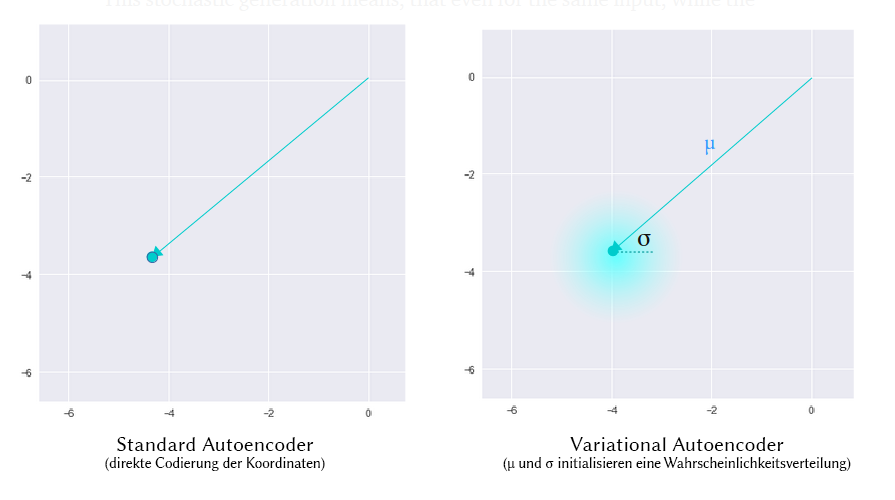
\includegraphics[width=0.75\textwidth,angle=0]{abb/VAE_muandsigma.png}
    \caption[VAE]{Unterschied im Encoding Autoencoder vs. VAE}
\end{figure}


\subsection{Generative Adversarial Networks (GAN)}\label{Generative Adversarial Networks (GAN)}

Dritter Unterabschnitt
